\documentclass[$if(fontsize)$$fontsize$,$endif$$if(lang)$$lang$,$endif$$if(papersize)$$papersize$,$endif$$for(classoption)$$classoption$$sep$,$endfor$]{$documentclass$}
$if(fontfamily)$
\usepackage{$fontfamily$}
$else$
\usepackage{lmodern}
$endif$

% Include pdfs
\usepackage{pdfpages}

% Continous footnote numbering
% \usepackage{chngcntr}

% Avoid widows and clubs
\clubpenalty10000
\widowpenalty10000
\interlinepenalty100
\displaywidowpenalty=10000
\interfootnotelinepenalty=10000
% keep figures where there are in the text
\usepackage{float}
\floatplacement{figure}{H}

% Overwrite \begin{figure}[htbp] with \begin{figure}[H]
\usepackage{float}
\let\origfigure=\figure
\let\endorigfigure=\endfigure
\renewenvironment{figure}[1][]{%
\origfigure[b]
}{%
\endorigfigure
}

% fix for pandoc 1.14
\providecommand{\tightlist}{%
  \setlength{\itemsep}{0pt}\setlength{\parskip}{0pt}}

% TP: hack to truncate list of figures/tables.
\usepackage{truncate}
\usepackage{caption}
\usepackage{tocloft}
% TP: end hack

$if(linestretch)$
\usepackage{setspace}
\setstretch{$linestretch$}
$endif$
\usepackage{amssymb,amsmath}
\usepackage{ifxetex,ifluatex}
% \usepackage{fixltx2e} % provides \textsubscript
\ifnum 0\ifxetex 1\fi\ifluatex 1\fi=0 % if pdftex
  \usepackage[T1]{fontenc}
  \usepackage[utf8]{inputenc}
$if(euro)$
  \usepackage{eurosym}
$endif$
\else % if luatex or xelatex
  \ifxetex
    \usepackage{mathspec}
    \usepackage{xltxtra,xunicode}
  \else
    \usepackage{fontspec}
  \fi
  \defaultfontfeatures{Mapping=tex-text,Scale=MatchLowercase}
  \newcommand{\euro}{€}
$if(mainfont)$
    \setmainfont{$mainfont$}
$endif$
$if(sansfont)$
    \setsansfont{$sansfont$}
$endif$
$if(monofont)$
    \setmonofont[Mapping=tex-ansi]{$monofont$}
$endif$
$if(mathfont)$
    \setmathfont(Digits,Latin,Greek){$mathfont$}
$endif$
\fi
% use upquote if available, for straight quotes in verbatim environments
\IfFileExists{upquote.sty}{\usepackage{upquote}}{}
% use microtype if available
\IfFileExists{microtype.sty}{%
\usepackage{microtype}
\UseMicrotypeSet[protrusion]{basicmath} % disable protrusion for tt fonts
}{}
$if(geometry)$
\usepackage[$for(geometry)$$geometry$$sep$,$endfor$]{geometry}
$endif$
$if(natbib)$
\usepackage{natbib}
\bibliographystyle{$if(biblio-style)$$biblio-style$$else$plainnat$endif$}
$endif$
$if(biblatex)$
\usepackage{biblatex}
$if(biblio-files)$
\bibliography{$biblio-files$}
$endif$
$endif$
$if(listings)$
\usepackage{listings}
$endif$
$if(lhs)$
\lstnewenvironment{code}{\lstset{language=Haskell,basicstyle=\small\ttfamily}}{}
$endif$
$if(highlighting-macros)$
$highlighting-macros$
$endif$
$if(verbatim-in-note)$
\usepackage{fancyvrb}
$endif$
$if(tables)$
\usepackage{longtable,booktabs}
$endif$
$if(graphics)$
\usepackage{graphicx}
\makeatletter
\def\maxwidth{\ifdim\Gin@nat@width>\linewidth\linewidth\else\Gin@nat@width\fi}
\def\maxheight{\ifdim\Gin@nat@height>\textheight\textheight\else\Gin@nat@height\fi}
\makeatother
% Scale images if necessary, so that they will not overflow the page
% margins by default, and it is still possible to overwrite the defaults
% using explicit options in \includegraphics[width, height, ...]{}
\setkeys{Gin}{width=\maxwidth,height=\maxheight,keepaspectratio}
$endif$
\ifxetex
  \usepackage[setpagesize=false, % page size defined by xetex
              unicode=false, % unicode breaks when used with xetex
              xetex]{hyperref}
\else
  \usepackage[unicode=true]{hyperref}
\fi
\hypersetup{breaklinks=true,
            bookmarks=true,
            pdfauthor={$author-meta$},
            pdftitle={$title-meta$},
            colorlinks=true,
            citecolor=$if(citecolor)$$citecolor$$else$blue$endif$,
            urlcolor=$if(urlcolor)$$urlcolor$$else$blue$endif$,
            linkcolor=$if(linkcolor)$$linkcolor$$else$magenta$endif$,
            pdfborder={0 0 0}}
\urlstyle{same}  % don't use monospace font for urls
$if(links-as-notes)$
% Make links footnotes instead of hotlinks:
\renewcommand{\href}[2]{#2\footnote{\url{#1}}}
$endif$
$if(strikeout)$
\usepackage[normalem]{ulem}
% avoid problems with \sout in headers with hyperref:
\pdfstringdefDisableCommands{\renewcommand{\sout}{}}
$endif$
\setlength{\parindent}{0pt}
\setlength{\parskip}{6pt plus 2pt minus 1pt}
\setlength{\emergencystretch}{3em}  % prevent overfull lines
$if(numbersections)$
\setcounter{secnumdepth}{5}
$else$
\setcounter{secnumdepth}{0}
$endif$
$if(verbatim-in-note)$
\VerbatimFootnotes % allows verbatim text in footnotes
$endif$
\usepackage[ngerman]{babel}

$for(header-includes)$
$header-includes$
$endfor$

\begin{document}
% Continous footnote numbering
% \counterwithout{footnote}{chapter}

\begin{titlepage}
    \begin{center}

      
\includegraphics[width=0.4\textwidth]{template/uzh_logo_d_pos.pdf}

        \vspace*{2.5cm}

        \huge
        {$title$}

        \vspace{0.5cm}

        \large
        {$subtitle$}

        \vspace{1.5cm}

        \Large
        {$author$}

        \normalsize
        {$studentnumber$}

        \vspace{1.5cm}

        \normalsize
        Masterarbeit\\
        zur Erlangung des akademischen Grades\\
        \textbf{Master of Arts UZH}\\
        der Philosophischen Fakultät\\
        der Universität Zürich

        \vfill

        \normalsize
        Referentin/Referent: {$supervisor$}\\
        $if(cosupervisor)$Betreuer/Betreuerin: {$cosupervisor$}\\$endif$

        \vspace{0.8cm}

        \normalsize
        {$institute$}\\
        Abgabedatum: {$date$}

    \end{center}
\end{titlepage}

$if(abstract)$
\clearpage\mbox{}\thispagestyle{empty}\clearpage
\renewcommand{\abstractname}{Abstract}
\begin{abstract}
$abstract$
\end{abstract}
$endif$

$if(abstract_other_lang_title)$
\renewcommand{\abstractname}{$abstract_other_lang_title$}
$endif$
$if(abstract_other_lang)$
\begin{abstract}
$abstract_other_lang$
\end{abstract}
$endif$

$if(thanks)$
\renewcommand{\abstractname}{Danksagung}
\begin{abstract}
$thanks$
\end{abstract}
\clearpage\mbox{}\thispagestyle{empty}\clearpage
% \pagestyle{empty}
% \thispagestyle{empty}
% \newpage
$endif$

$for(include-before)$
$include-before$
$endfor$

\pagenumbering{roman}                   % roman page number for toc
\setcounter{page}{1}

$if(toc)$
{
\hypersetup{linkcolor=black}
\setcounter{tocdepth}{$toc-depth$}
\tableofcontents
}

$endif$
$if(lot)$
\newpage
\listoftables
$endif$
$if(lof)$
\newpage
\listoffigures
$endif$

\clearpage\mbox{}\thispagestyle{empty}\clearpage
%\clearpage
\pagenumbering{arabic}                  % Start text with arabic 1
\setcounter{page}{1}

$body$

$if(natbib)$
$if(biblio-files)$
$if(biblio-title)$
$if(book-class)$
\renewcommand\bibname{$biblio-title$}
$else$
\renewcommand\refname{$biblio-title$}
$endif$
$endif$
\bibliography{$biblio-files$}

$endif$
$endif$
$if(biblatex)$
\printbibliography$if(biblio-title)$[title=$biblio-title$]$endif$

$endif$
$for(include-after)$
$include-after$
$endfor$

\newpage
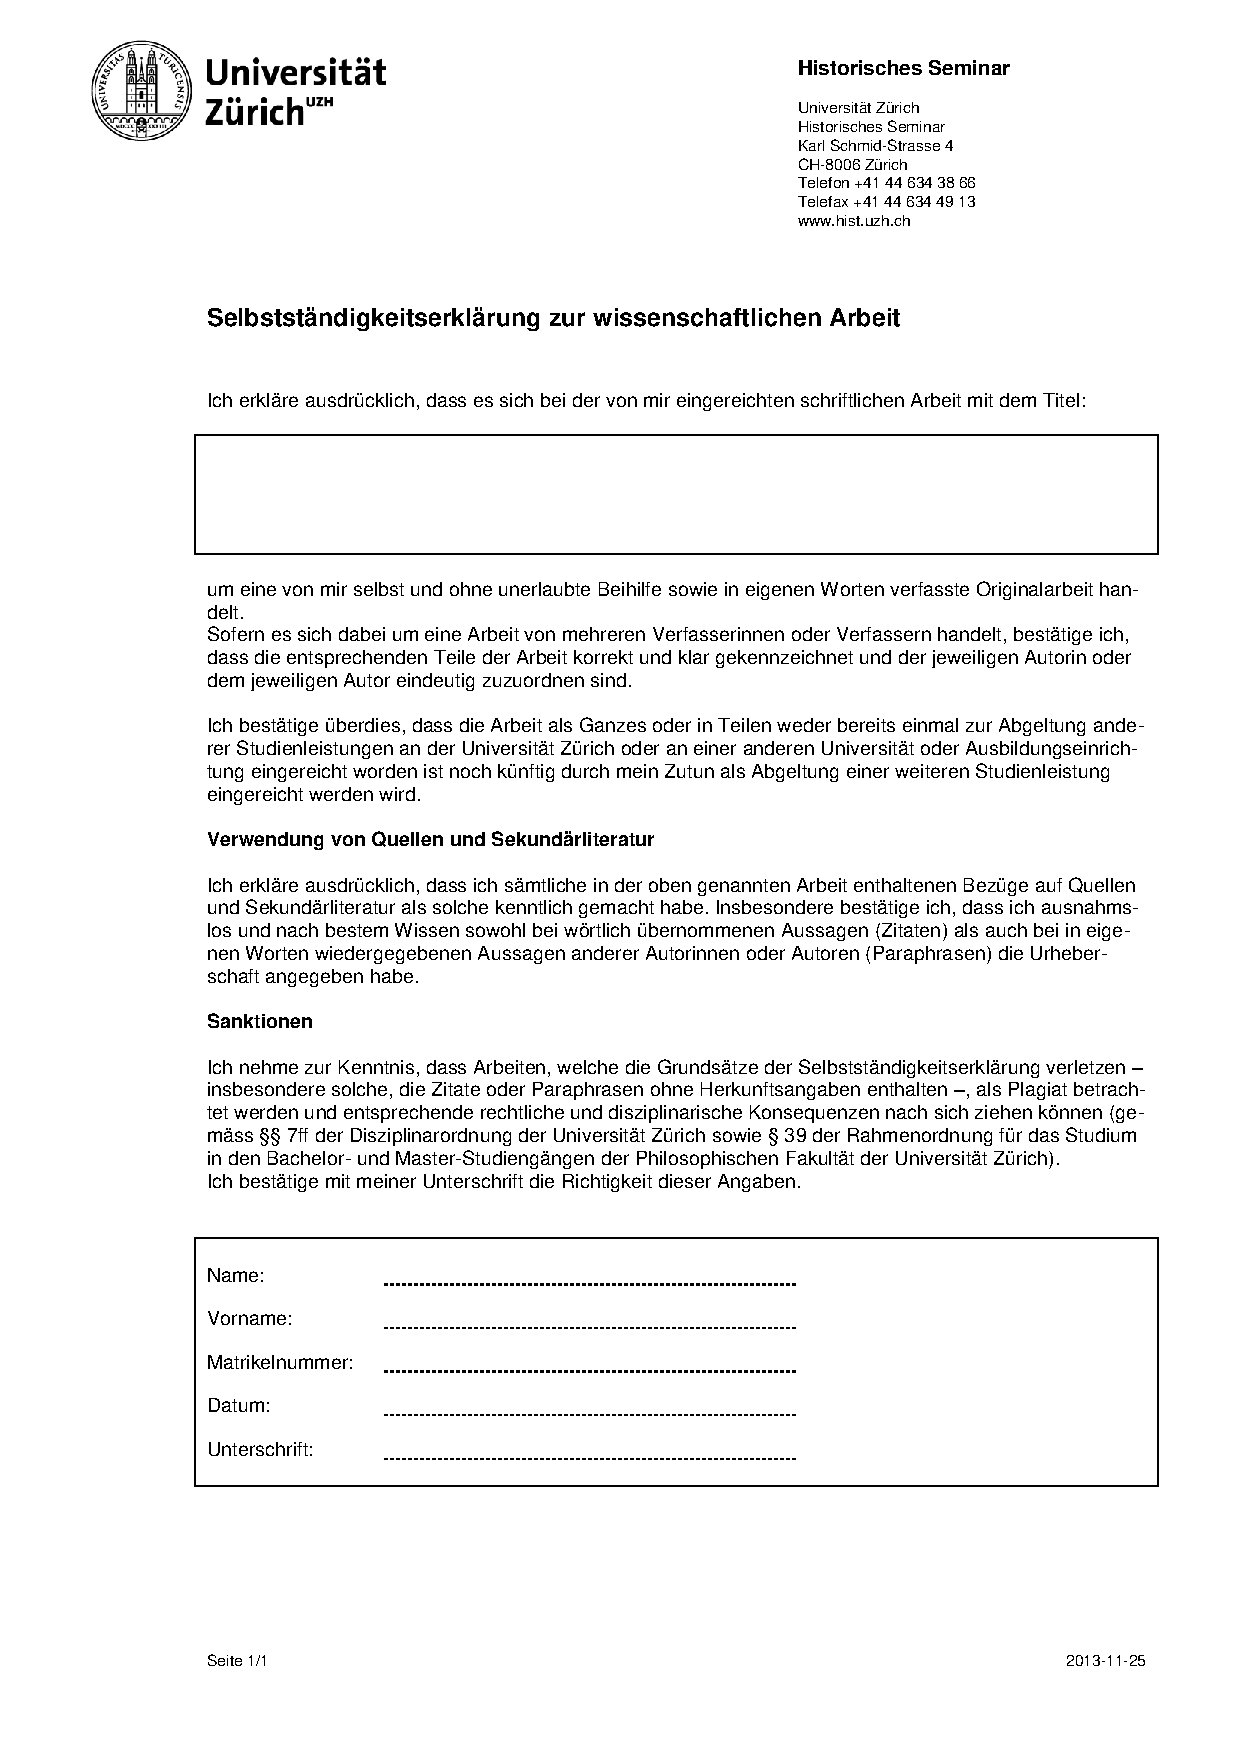
\includepdf[pages=-]{./addendum/selbststaendigkeitserklaerung.pdf}

\end{document}
